\documentclass{standalone}
\usepackage{tikz}
\usetikzlibrary{positioning, calc}

\begin{document}

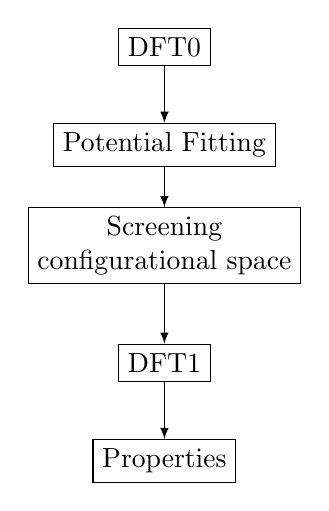
\begin{tikzpicture}[every node/.style={anchor=center, draw, align=center}]
  \node (A) at (0,0) {DFT0};
  \node  (B) at ( $(A.south) + (0, -1cm)$ ) {Potential Fitting};
  \node  (C) at ( $(B.south) + (0, -1cm)$ ) {Screening\\configurational space};
  \node  (D) at ( $(C.south) + (0, -1cm)$ ) {DFT1};
  \node  (E) at ( $(D.south) + (0, -1cm)$ ) {Properties};

  \path[draw, -latex] (A) -- (B);
  \path[draw, -latex] (B) -- (C);
  \path[draw, -latex] (C) -- (D);
  \path[draw, -latex] (D) -- (E);
\end{tikzpicture}

\end{document}

